%==========================================================
% Preamble
%==========================================================
% Fonts/languages
\documentclass[english,final,t]{beamer}
%\usepackage[orientation=portrait,size=custom,width=91.44,height=121.92,scale=1.6]{beamerposter} % 3' x 4' portait poster, adjust scale as desired
\usepackage[orientation=landscape,size=custom,width=121.92,height=91.44,scale=1.6]{beamerposter} % 4' x 3' landscape poster, adjust scale as needed
\usepackage[T1]{fontenc}
\usepackage[latin9]{inputenc}
\usepackage{lmodern}          % allows LaTeX to make any arbitrary font size
\usepackage{babel}            % For bibliographies
%\usepackage{mathpazo}         % For Palatino font
%\usepackage{mathptmx}        % For Times New Roman font
%\usefonttheme{serif}          % To have a serif font (instead of Beamer's default sans serif)

\usepackage[scaled]{beramono}  % Load typewriter font first, since Arial doesn't have one
\usepackage{helvet}            % For Arial font
\renewcommand{\familydefault}{\sfdefault}

% Beamer Theme
\mode<presentation>
{\usetheme{PosterExample}}
\setbeamertemplate{navigation symbols}{}                   % remove annoying navigation symbols
%\setbeamertemplate{footline}{}                             % remove footer line
\setbeamercovered{transparent}

% Useful Packages
\usepackage{babel}                                                 % For multilingual output
\usepackage{amsthm}                                                % For detailed theorems
\usepackage{amssymb}                                               % For fancy math symbols
\usepackage{amsmath}                                               % For awesome equations/equation arrays
\usepackage{float}                                                 % For improved float manipulation
\usepackage{prettyref}                                             % For pretty references
\usepackage{array}                                                 % For tubular tables
\usepackage{longtable}                                             % For long tables
\usepackage[flushleft]{threeparttable}                             % For three-part tables
\usepackage{multicol}                                              % For multi-column cells
\usepackage{graphicx}                                              % For shiny pictures
\usepackage{subfig}                                                % For sub-shiny pictures
\usepackage{enumerate}                                             % For cusomtizable lists
\usepackage{outline}                                               % For an outline environment (similar to enumerate, but can go six levels deep)
\usepackage{pdflscape}                                             % For landscape-oriented pages
%\usepackage{pstricks,pst-node,pst-plot,pst-circ,pst-tree,moredefs} % For trees
%\usepackage{tikz,pgfplots}                                         % For tikz figures
%\pgfplotsset{compat=1.7}
%\pgfplotsset{scaled y ticks=base 10:2}

% Bib
%\usepackage[authoryear]{natbib}                                    % Bibliography
%\renewcommand{\bibsection}{\subsubsection*{\bibname } }            % Allows Bibliographies in Beamer
%\usepackage{url}                                                   % Allows urls in bib

% Links
%\usepackage{hyperref}                                              % Always add hyperref (almost) last
%\hypersetup{unicode=true,bookmarksnumbered=true,bookmarksopen=true,bookmarksopenlevel=4,
% breaklinks=true,pdfborder={0 0 0},colorlinks=false,citecolor=black,filecolor=black,linkcolor=black,urlcolor=black}
%\hypersetup{unicode=true,breaklinks=true,pdfborder={0 0 0}}

% Misc
\listfiles                                                         % List files in LaTeX log
%\graphicspath{{figures/}}                                          % Set file path to graphics

\title{\huge Mechanisms Underlying the City Size Wage Premium}
\author[Ransom]{Tyler Ransom}
\institute[Duke University]{Department of Economics, Duke University}
\date[May 16, 2013]{May 16, 2013}


%%%%%%%%%%%%%%%%%%%%%%%%%%%%%%%%%%%%%%%%%%%%%%%%%%%%%%%%%%%%%%%%%%%%%%%%%%%%%%%%%%%%%%%%%%%%%%%%%%%%%%%%%%%%
%%%%%%%%%%%%%%%%%%%%%%%%%%%%%%%%%%%%%%%%%%%%%%%%%%%%%%%%%%%%%%%%%%%%%%%%%%%%%%%%%%%%%%%%%%%%%%%%%%%%%%%%%%%%
\begin{document}
\begin{frame}{}
\begin{part}{}
  \begin{columns}[t]
    \begin{column}{.22\linewidth}

      %%%%%%%%%%%%%%%%%%%%%%%%%%%%%%%%%%%%%%%%%%%%%%%%%%%%%%%%%%%%%%%%%%%%%%%%%%%%%%%%%%%%%%%%%%%%%%%%%%%%%%%%%%%%

      \begin{block}{Introduction}
        \begin{itemize}
				\item \textbf{Agglomeration economies}: efficiency gains from density of economic activity
				\item These gains impact both firms and workers
				\item Literature has identified that \textbf{workers in larger cities earn higher wages}
				\item My research seeks to improve the understanding for why this occurs
        \end{itemize}
      \end{block}
			
      \begin{block}{Research Question}
        \begin{itemize}
				\item \textbf{Quantify competing explanations for city size wage premium:}
        \end{itemize}
				\begin{enumerate}
				\item Sorting on observed and unobserved skill
				\item Compensating differentials for locational amenities
				\item True productivity premium arising from local productivity differences
				\end{enumerate}
      \end{block}
    \end{column}

      %%%%%%%%%%%%%%%%%%%%%%%%%%%%%%%%%%%%%%%%%%%%%%%%%%%%%%%%%%%%%%%%%%%%%%%%%%%%%%%%%%%%%%%%%%%%%%%%%%%%%%%%%%%%

    \begin{column}{.44\linewidth}
      \begin{block}{Motivating evidence: characteristics by city size category}
			\vspace{1ex}
      \centering
        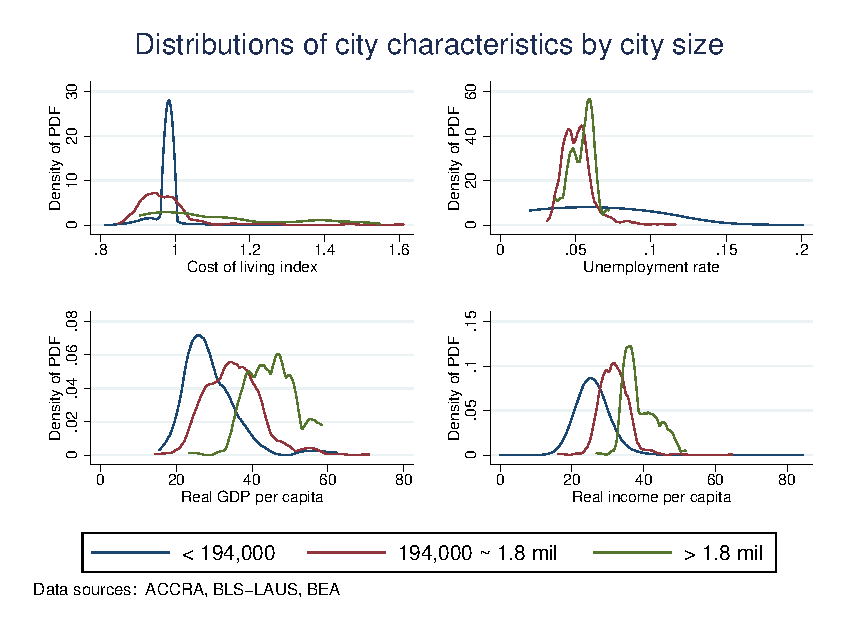
\includegraphics[width=.9\linewidth]{alldist.eps}
        \vspace{-1ex}
      \end{block}
    \end{column}

    %%%%%%%%%%%%%%%%%%%%%%%%%%%%%%%
    
    \begin{column}{.22\linewidth}

      \begin{block}{Research method}
        \begin{itemize}
        \item Dynamic search model
        \item Individuals choose location and labor force status that will maximize present value of expected utility
				\item Wage enters utility if employed
        \item Location amenities enter utility regardless of job search outcome
        %\item init
        \end{itemize}
        \vspace{1ex}
      \end{block}

      \begin{block}{Preliminary results}
        \begin{itemize}
        \item Large amount of sorting on observable characteristics: (2) vs. (1)
				\item Even larger amount of sorting on unobservables: (3) vs. (1)
        \item Evidence of preferences for amenities: (4)-(6) vs. (1)-(3)
        %\item Need to model the location choice to properly interpret these results
        \item Need to carefully control for effects of selection and preferences on wage estimates to properly interpret results
        \end{itemize}
        \vspace{-1ex}
      \end{block}
%%%%%%%%%%%%%%%%%%%%%%%%%%%%%%%%%%%%%%%%%%%%%%%%%%%%%%%

    \end{column}
  \end{columns}
\end{part}
\vspace{2ex}
\begin{part}{}

  \begin{columns}[t]
    \begin{column}{.22\linewidth}

      %%%%%%%%%%%%%%%%%%%%%%%%%%%%%%%%%%%%%%%%%%%%%%%%%%%%%%%%%%%%%%%%%%%%%%%%%%%%%%%%%%%%%%%%%%%%%%%%%%%%%%%%%%%%

      \begin{block}{Data}
        \begin{itemize}
				\item \textbf{2004 Survey of Income and Program Participation (SIPP)}
				\item Individual-level data including:
				\item[$\bullet$] monthly earnings
				\item[$\bullet$] monthly labor force status
				\item[$\bullet$] migration history
				\vspace{3ex}
				\item \textbf{Estimation subsample:}
        \item[$\bullet$] Non-Hispanic white males aged 18-60 who have completed highest level of schooling
				\item[$\bullet$] $N=24,261$
				\vspace{3ex}
        \item \textbf{Locational characteristics:}
        \item[$\bullet$] population (2000 Census)
				\item[$\bullet$] prices (ACCRA)
				\item[$\bullet$] productivity (BEA)
				\item[$\bullet$] labor statistics (BLS-LAUS)
        \end{itemize}
      \end{block}
    \end{column}

      %%%%%%%%%%%%%%%%%%%%%%%%%%%%%%%%%%%%%%%%%%%%%%%%%%%%%%%%%%%%%%%%%%%%%%%%%%%%%%%%%%%%%%%%%%%%%%%%%%%%%%%%%%%%
			
		\begin{column}{.44\linewidth}      
      \begin{block}{Results: log wage regressions}
			\begin{small}
			\begin{center}
			\begin{threeparttable}
			\begin{tabular}{cccc|ccc}
			\hline
			& \multicolumn{3}{c|}{\emph{Temporally deflated wages only:}} & \multicolumn{3}{c}{\emph{Spatially and temporally deflated wages:}} \\
			& \multicolumn{3}{c|}{\emph{(Worker productivity)}} & \multicolumn{3}{c}{\emph{(Worker productivity less amenities)}} \\
			Variable & (1) & (2) & (3) & (4) & (5) & (6) \\
			\hline
			medium city & 0.1829*** & 0.1003*** & -0.0292*** & 0.1637*** & 0.0851*** & -0.0315*** \\
			 & (0.0025) & (0.0022) & (0.0111) & (0.0025) & (0.0022) & (0.0112) \\
			large city & 0.3773*** & 0.2370*** & 0.0135 & 0.2182*** & 0.0857*** & -0.1234*** \\
			 & (0.0026) & (0.0023) & (0.0127) & (0.0026) & (0.0023) & (0.0129) \\
			age &  & 0.0448*** & 0.0112* &  & 0.0391*** & 0.0051 \\
			 &  & (0.0012) & (0.0061) &  & (0.0012) & (0.0061) \\
			experience &  & 0.0092*** & 0.0454*** &  & 0.0128*** & 0.0512*** \\
			 &  & (0.0006) & (0.0042) &  & (0.0007) & (0.0042) \\
			tenure &  & 0.0223*** & 0.0026*** &  & 0.0222*** & 0.0022*** \\
			 &  & (0.0003) & (0.0008) &  & (0.0003) & (0.0008) \\
			years of education &  & 0.0877*** &  &  & 0.0853*** &  \\
			 &  & (0.0005) &  &  & (0.0005) &  \\
			\hline
			industry/occupation dummies &  & $\checkmark$ & $\checkmark$ &  & $\checkmark$ & $\checkmark$ \\
			individual fixed effects &  &  & $\checkmark$ &  &  & $\checkmark$ \\
			person-months & 398,447 & 398,447 & 398,447 & 398,447 & 398,447 & 398,447 \\
			persons & 16,070 & 16,070 & 16,070 & 16,070 & 16,070 & 16,070 \\
			R-squared & 0.050 & 0.323 & 0.756 & 0.018 & 0.291 & 0.745 \\
			\hline
			\end{tabular}
			Dependent variable is log wage. Robust standard errors in parentheses. Regressions also include an intercept and quadratic terms for age, experience, and tenure.
			*** p<0.01;
			** p<0.05;
			* p<0.10
			\end{threeparttable}
			\end{center}
			\end{small}
      \end{block}
    \end{column}

    %%%%%%%%%%%%%%%%%%%%%%%%%%%%%%%
    
    \begin{column}{.22\linewidth}

      \begin{block}{Conclusion}
        \begin{itemize}
				\item There is a sizable, monotonic city size wage premium that persists even after controlling for cost of living and a variety of human capital and local productivity measures
				\item The structural model appropriately treats selection of skilled workers into cities
				\item Simulations of the model will reveal the relative importance of each of the sources contributing to the wage premium
        \end{itemize}
        \vspace{3ex}
      \end{block}
			
      \vspace{-3ex}
      \begin{block}{Acknowledgments}
      \begin{scriptsize}
			\begin{itemize}
      \item[] \textbf{Thanks to:}
			\item Peter Arcidiacono and seminar participants at Duke University and Georgia State University for helpful comments; funding from NSF Grant SES-11-31897
			\end{itemize}
			\begin{itemize}
			\item[] \textbf{Disclaimer:}
			\item Any opinions and conclusions expressed herein are my own and do not necessarily represent the views of the U.S. Census Bureau
			\item All results have been reviewed to ensure that no confidential information is disclosed.
			\end{itemize}
      \end{scriptsize}
      \end{block}
			
%%%%%%%%%%%%%%%%%%%%%%%%%%%%%%%%%%%%%%%%%%%%%%%%%%%%%%%

    \end{column}
  \end{columns}
\end{part}
\end{frame}

\end{document}
